\documentclass{beamer}

\usepackage[utf8x]{inputenc}
\usepackage{graphicx}
\usepackage{amsthm,amssymb,amsbsy,amsmath,amsfonts,amssymb,amscd}
\usepackage{dsfont}
\usepackage{array}
\newcolumntype{N}{@{}m{2pt}@{}}
\usepackage{tikz}
%\usetikzlibrary{arrows}
%\tikzstyle{block}=[draw opacity=0.7,line width=1.4cm]

\input{../style.tex} 

\DeclareMathOperator*{\Var}{var}
\DeclareMathOperator*{\E}{E}
\DeclareMathOperator*{\Cov}{cov}
\newcommand\PR[1]{\mathrm{P}\left(#1 \right)}
\newcommand\PS[1]{{\langle #1 \rangle}_\mathcal{H}}
\newcommand\PSi[2]{{ \left \langle #1 \right \rangle}_{\! #2}}
\newcommand\N[1]{{|| #1 ||}_\mathcal{H}}
\newcommand\Ni[2]{{|| #1 ||}_{\! #2}}
\newcommand\dx{\, \mathrm{d}}
\newcommand\textequal{\rule[.4ex]{4pt}{0.4pt}\llap{\rule[.7ex]{4pt}{0.4pt}}}
\newcommand{\argmin}{\operatornamewithlimits{argmin}}
\makeatletter
\newcommand{\shorteq}{%
  \settowidth{\@tempdima}{a}% Width of hyphen
  \resizebox{\@tempdima}{\height}{=}%
}
\makeatother

\title[Majeure Data Science -- Surrogate models and GPR]{\texorpdfstring{ \small Surrogate models and Gaussian Process regression -- lecture 1/5 \\ \vspace{3mm} \LARGE Surrogate models in engineering}{}}
\author[Mines St-\'Etienne ]{Mines St-\'Etienne -- Majeure Data Science -- 2016/2017}
\institute{\texorpdfstring{Nicolas Durrande (durrande@emse.fr)}{}}
\date{\null}

%%%%%%%%%%%%%%%%%%%%%%%%%%%%%%%%%%%%%%%%%%%%%%%%%%%%%%
%%%%%%%%%%%%%%%%%%%%%%%%%%%%%%%%%%%%%%%%%%%%%%%%%%%%%%
%%%%%%%%%%%%%%%%%%%%%%%%%%%%%%%%%%%%%%%%%%%%%%%%%%%%%%
\begin{document}

%%%%%%%%%%%%%%%%%%%%%%%%%%%%%%%%%%%%%%%%%%%%%%%%%%%%%%
\begin{frame}
  \titlepage
\end{frame}

%%%%%%%%%%%%%%%%%%%%%%%%%%%%%%%%%%%%%%%%%%%%%%%%%%%%%%
%%%%%%%%%%%%%%%%%%%%%%%%%%%%%%%%%%%%%%%%%%%%%%%%%%%%%%
\section[Intro.]{Introduction}
\subsection{}

%%%%%%%%%%%%%%%%%%%%%%%%%%%%%%%%%%%%%%%%%%%%%%%%%%%%%%
\begin{frame}{}
\structure{Context:}\\
\vspace{0.5cm}
The aim of this module is to introduce a framework dedicated to the study of functions that are \textbf{costly to evaluate}.\\
\vspace{5mm}
Detail of the courses:
\begin{itemize}
	\item Surrogate models and Gaussian process regression (N. Durrande, A. Lopez Lopera)
	\item Application to sensitivity analysis (E. Padonou)
	\item Optimization (Y. Richet, N. Garland)
	\item Helicopter project (N. Durrande, A. Lopez Lopera).
\end{itemize}
\end{frame}


%%%%%%%%%%%%%%%%%%%%%%%%%%%%%%%%%%%%%%%%%%%%%%%%%%%%%%
\begin{frame}{}
The project will be on the optimization of paper helicopters:\\
\vspace{3mm} \
\hspace{-5mm}\includegraphics[height=6cm]{figures/latexdraw/helico} \quad \includegraphics[height=5.8cm]{figures/helicopter2}
\vspace{4mm}
\begin{center}
	\textbf{What value of $(a_l,\ w_l,\ t_l,\ w_w)$ gives the longest falling time?}
\end{center}
\end{frame}

%%%%%%%%%%%%%%%%%%%%%%%%%%%%%%%%%%%%%%%%%%%%%%%%%%%%%%
\begin{frame}{}
\centering
\vspace{-2.5cm}\includegraphics[height=17cm]{figures/EDT_DataScience_UP4_2016.pdf}
\end{frame}

%%%%%%%%%%%%%%%%%%%%%%%%%%%%%%%%%%%%%%%%%%%%%%%%%%%%%%
\begin{frame}{}

\vspace{0.5cm}
\structure{Course material:}\\
\begin{itemize}
	\item Handout
	\item Campus
	\item github: https://github.com/NicolasDurrande/EMSE_Gaussian_process_models
\end{itemize}

\vspace{0.5cm}
\structure{Marking:}\\
\begin{itemize}
	\item A 2h exam at the end of the course (60\% of the mark).
	\item A report on the helicopter project (40\% of the mark).
\end{itemize}

\vspace{5mm}
\structure{Presence:}
\begin{itemize}
	\item attending classes and lab session is mandatory.
	\item after one unjustified absence : -0.5pts on the mark per unjustified absence
\end{itemize}
\end{frame}

%%%%%%%%%%%%%%%%%%%%%%%%%%%%%%%%%%%%%%%%%%%%%%%%%%%%%%
\begin{frame}{}
Why is presence important:
\begin{center}
  \includegraphics[height=6cm]{figures/notes_vs_abs.pdf}
\end{center}
\end{frame}

%%%%%%%%%%%%%%%%%%%%%%%%%%%%%%%%%%%%%%%%%%%%%%%%%%%%%%
\begin{frame}{}
Outline of today's lecture
\vspace{0.2cm}
\begin{itemize}
	\item Why (and when) statistical models can be useful in engineering?
	\item Some typical methods:
	\begin{itemize}
		\item Linear regression
		\item Polynomial Chaos
		\item Neural networks
		\item Gaussian process regression (Kriging)
	\end{itemize}
\end{itemize}
\end{frame}

%%%%%%%%%%%%%%%%%%%%%%%%%%%%%%%%%%%%%%%%%%%%%%%%%%%%%%
%%%%%%%%%%%%%%%%%%%%%%%%%%%%%%%%%%%%%%%%%%%%%%%%%%%%%%
\section[Surrogate models]{Why are surrogate models relevant in engineering?}
\subsection{}

%%%%%%%%%%%%%%%%%%%%%%%%%%%%%%%%%%%%%%%%%%%%%%%%%%%%%%
\begin{frame}{}
There is a wide variety of situations where getting data is extremely expensive.
\begin{itemize}
	\item real world experiments
	\item destructive tests
	\item prototyping
	\item numerical experiments
\end{itemize}
\end{frame}

%%%%%%%%%%%%%%%%%%%%%%%%%%%%%%%%%%%%%%%%%%%%%%%%%%%%%%
\begin{frame}{}
\begin{exampleblock}{Example: real world experiments}
\begin{center}
\includegraphics[height=5cm]{figures/drilling}
\end{center}
\end{exampleblock}
\end{frame}

%%%%%%%%%%%%%%%%%%%%%%%%%%%%%%%%%%%%%%%%%%%%%%%%%%%%%%
\begin{frame}{}
\begin{exampleblock}{Example: Destructive tests}
\begin{center}
\includegraphics[height=5cm]{figures/crash-test}
\end{center}
\end{exampleblock}
\end{frame}

%%%%%%%%%%%%%%%%%%%%%%%%%%%%%%%%%%%%%%%%%%%%%%%%%%%%%%
\begin{frame}{}
\begin{exampleblock}{Example: Prototyping of a boat shape}
\begin{center}
\includegraphics[height=3.5cm]{figures/carene} \qquad \includegraphics[height=3.5cm]{figures/carene2}
\end{center}
Knowing the drag for a given design requires costly experiments
\end{exampleblock}
\end{frame}

%%%%%%%%%%%%%%%%%%%%%%%%%%%%%%%%%%%%%%%%%%%%%%%%%%%%%%
\begin{frame}{}
\begin{exampleblock}{In practice: Numerical experiments are extremely common}
\begin{center}
\includegraphics[height=2.8cm]{figures/waterflow} \qquad \includegraphics[height=4.2cm]{figures/image15}
\end{center}
They are less expensive but can be very time consuming!
\end{exampleblock}
\end{frame}

%%%%%%%%%%%%%%%%%%%%%%%%%%%%%%%%%%%%%%%%%%%%%%%%%%%%%%
\begin{frame}{}
\begin{exampleblock}{Example in medecine}
Deep brain simulation is an effective method to treat patients with Parkinson Desease
\begin{center}
\includegraphics[height=3.5cm]{figures/DeepBrainSimulation.png} \qquad \includegraphics[height=3.5cm]{figures/DBSelectrode.png} \qquad \includegraphics[height=3.5cm]{figures/DBSactivation}
\end{center}
\begin{flushright}
{\small \emph{source:} Seminar from M. Alvarez (Univ. Tech de Pereira, Colombia) at Mines St-\'Etienne, 2016.}
\end{flushright}
\end{exampleblock}
\end{frame}

%%%%%%%%%%%%%%%%%%%%%%%%%%%%%%%%%%%%%%%%%%%%%%%%%%%%%%
\begin{frame}{}
\begin{exampleblock}{Example in medecine}
Computing the volume of tissus activated required two numerical simulator
\begin{center}
\includegraphics[height=5cm]{figures/DBSmodels.png}
\end{center}
\begin{flushright}
{\small \emph{source:} Seminar from M. Alvarez (Univ. Tech de Pereira, Colombia) at Mines St-\'Etienne, 2016.}
\end{flushright}
\end{exampleblock}
\end{frame}

%%%%%%%%%%%%%%%%%%%%%%%%%%%%%%%%%%%%%%%%%%%%%%%%%%%%%%
\begin{frame}{}
In all these cases, the variable of interest can be seen as a function of the input parameters
$$ y = f(x). $$
where $f$ is a \textbf{costly to evaluate function}. \\
\vspace{5mm}
In the following, we will assume that 
\begin{itemize}
	\item $x \in \mathds{R}^d$: There are many input parameters
	\item $y \in \mathds{R}$: The output is a scalar.
\end{itemize}
\end{frame}

%%%%%%%%%%%%%%%%%%%%%%%%%%%%%%%%%%%%%%%%%%%%%%%%%%%%%%
\begin{frame}{}
The fact that $f$ is \textbf{costly to evaluate} changes a lot of things...\\
\vspace{5mm}
\structure{1. Representing the function is not possible...}\\
\vspace{5mm}
\begin{center}
\includegraphics[height=3.2cm]{figures/ink_f} \includegraphics[height=3.2cm]{figures/Rightarrow} \includegraphics[height=3.2cm]{figures/ink_fX}
\end{center}
\end{frame}

%%%%%%%%%%%%%%%%%%%%%%%%%%%%%%%%%%%%%%%%%%%%%%%%%%%%%%
\begin{frame}{}
The fact that $f$ is \textbf{costly to evaluate} changes a lot of things...\\
\vspace{5mm}
\structure{2. Computing integrals is not possible...}\\
\vspace{5mm}
\begin{center}
\includegraphics[height=4.5cm]{figures/ink_fX}
\end{center}
What is the mean value of $f$?
\end{frame}

%%%%%%%%%%%%%%%%%%%%%%%%%%%%%%%%%%%%%%%%%%%%%%%%%%%%%%
\begin{frame}{}
The fact that $f$ is \textbf{costly to evaluate} changes a lot of things...\\
\vspace{5mm}
\structure{3. Uncertainty propagation is not possible...}\\
\vspace{5mm}
\begin{center}
\includegraphics[height=3.2cm]{figures/ink_unprogf} \includegraphics[height=3.2cm]{figures/Rightarrow} \includegraphics[height=3.2cm]{figures/ink_unprogfX}
\end{center}
\end{frame}

%%%%%%%%%%%%%%%%%%%%%%%%%%%%%%%%%%%%%%%%%%%%%%%%%%%%%%
\begin{frame}{}
The fact that $f$ is \textbf{costly to evaluate} changes a lot of things...\\
\vspace{5mm}
\structure{4. Sensitivity analysis is not possible...}\\
\vspace{5mm}
\begin{center}
\includegraphics[height=4.5cm]{figures/ink_as2}
\end{center}
\end{frame}

%%%%%%%%%%%%%%%%%%%%%%%%%%%%%%%%%%%%%%%%%%%%%%%%%%%%%%
\begin{frame}{}
The fact that $f$ is \textbf{costly to evaluate} changes a lot of things...\\
\vspace{5mm}
\structure{5. Optimisation is also tricky...}\\
\vspace{5mm}
\begin{center}
\includegraphics[height=4.5cm]{figures/ink_fX}
\end{center}
\end{frame}

%%%%%%%%%%%%%%%%%%%%%%%%%%%%%%%%%%%%%%%%%%%%%%%%%%%%%%
\begin{frame}{}
Another example of scattered data is the coupling of solvers with different physics 
\begin{example}
Fluid-structure interaction in aeroelasticity:
\begin{center}
\includegraphics[height=3.5cm]{figures/wenland}
\end{center}
{\small \hfill \emph{source:} H. Wendland, \emph{Scattered data approximation}. Vol. 17. Cambridge university press, 2004.}
\end{example}
\end{frame}


% %%%%%%%%%%%%%%%%%%%%%%%%%%%%%%%%%%%%%%%%%%%%%%%%%%%%%%
% %%%%%%%%%%%%%%%%%%%%%%%%%%%%%%%%%%%%%%%%%%%%%%%%%%%%%%
% \section[Surrogate models]{Surrogate models}
% \subsection{}

%%%%%%%%%%%%%%%%%%%%%%%%%%%%%%%%%%%%%%%%%%%%%%%%%%%%%%
\begin{frame}{}
The principle of statistical modelling is to use the data to build a mathematical approximation of the function. 
\begin{center}
\includegraphics[height=4.5cm]{figures/ink_m}
\end{center}
The model can then be used to answer all previous questions
\end{frame}

%%%%%%%%%%%%%%%%%%%%%%%%%%%%%%%%%%%%%%%%%%%%%%%%%%%%%%
\begin{frame}{}
Of course, there is a difference between $f$ and $m$...
\begin{center}
\includegraphics[height=5cm]{figures/ink_mf}
\end{center}
\end{frame}

%%%%%%%%%%%%%%%%%%%%%%%%%%%%%%%%%%%%%%%%%%%%%%%%%%%%%%
\begin{frame}{}
\textbf{\structure{Model validation}} is always of upper importance.\\ 
\vspace{3mm}
The goodness of fit can be measured by the \textbf{mean square error}:

\begin{columns}[c]
\column{4cm}
\begin{equation*}
MSE =  \frac{1}{n} \sum_i \big(f(t_i)-m(t_i) \big)^2
\end{equation*}
\column{5cm}
\begin{center}
  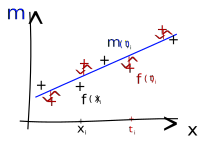
\includegraphics[height=4cm]{figures/ink_MSE}
\end{center}
\end{columns}
\vspace{2mm}
where $T = (t_1, \dots,t_n)$ is a set of test points. If no test set is available, one can use \textbf{cross validation} methods.
\end{frame}

%%%%%%%%%%%%%%%%%%%%%%%%%%%%%%%%%%%%%%%%%%%%%%%%%%%%%%
\begin{frame}{}
What about \textbf{statistical models}? \\We want to be able to quantify the model error:
\begin{center}
\includegraphics[height=5cm]{figures/ink_mconfint}
\end{center}
The confidence intervals can be used to obtain a \textbf{measure of uncertainty on the value of interest}.
\end{frame}

%%%%%%%%%%%%%%%%%%%%%%%%%%%%%%%%%%%%%%%%%%%%%%%%%%%%%%
\begin{frame}{}
In the sequel, we will use the following notations : 
\begin{itemize}
	\item The set of observation points will be represented by a $n \times d$ matrix $X=(X_1, ..., X_n)^t$
	\item The vector of observations will be denoted by $F$ : $F_i=f(X_i)$ (or $F=f(X)$).
\end{itemize}
\vspace{5mm}
We will now introduce various types of surrogate models:
\begin{columns}[t]
\column{5cm}
\begin{itemize}
	\item linear regression
	\item polynomial chaos
\end{itemize}
\column{5cm}
\begin{itemize}
	\item neural networks
	\item Gaussian process regression
\end{itemize}
\end{columns}
\end{frame}

%%%%%%%%%%%%%%%%%%%%%%%%%%%%%%%%%%%%%%%%%%%%%%%%%%%%%%
%%%%%%%%%%%%%%%%%%%%%%%%%%%%%%%%%%%%%%%%%%%%%%%%%%%%%%
\section{Linear Regression}
\subsection{}

%%%%%%%%%%%%%%%%%%%%%%%%%%%%%%%%%%%%%%%%%%%%%%%%%%%%%%
\begin{frame}{}
\textbf{Linear regression} is probably the most commonly used statistical model.\\ \vspace{3mm}
Given a set of basis functions $B=(b_0, \dots, b_p)$, we assume that the observations come from the probabilistic model
$$ F = B(X) \beta  + \varepsilon \qquad \qquad \left( \text{i.e. } F_i = \sum_{k=1}^p \beta_k b_k(X_i) + \varepsilon_i \right) $$
where the vector $\beta$ is unknown and the $\varepsilon_i$ are independent and identically distributed.
\end{frame}

%%%%%%%%%%%%%%%%%%%%%%%%%%%%%%%%%%%%%%%%%%%%%%%%%%%%%%
\begin{frame}{}
If we consider a model of the form 
$$m(x) = B(x) \hat{\beta}$$
the prediction error (Residual Sum of Square) is given by 
$$RSS = (B(X) \hat{\beta}  - F)^t(\hat{\beta} B(X) - F)  \qquad \qquad \left( \text{i.e. } \sum_{k=1}^n ( B(X_i) \hat{\beta} - F_i)^2\right)$$ 

Finding the optimal value of $\hat{\beta}$ means minimizing a quadratic form. This can be done analytically and we obtain $\hat{\beta} = (B(X)^t B(X))^{-1} B(X)^t F$.\\
\vspace{3mm}
The associated linear regression model is thus
$$m(x) = B(x) (B(X)^t B(X))^{-1} B(X)^t F.$$
\end{frame}

%%%%%%%%%%%%%%%%%%%%%%%%%%%%%%%%%%%%%%%%%%%%%%%%%%%%%%
\begin{frame}{}
\begin{example}
	If we consider the following observations: 
\begin{center}
  \includegraphics[height=5cm]{figures/R/linreg_0}
\end{center}
\end{example}
\end{frame}

%%%%%%%%%%%%%%%%%%%%%%%%%%%%%%%%%%%%%%%%%%%%%%%%%%%%%%
\begin{frame}{}
\begin{example}
	and a set of 3 basis functions:
	 $$b_0(x)=1,\ b_1(x)=x,\ b_2(x)=x^2$$
\begin{center}
  \includegraphics[height=5cm]{figures/R/linreg_1}
\end{center}
\end{example}
\end{frame}

%%%%%%%%%%%%%%%%%%%%%%%%%%%%%%%%%%%%%%%%%%%%%%%%%%%%%%
\begin{frame}{}
\begin{example}
We obtain $\hat{\beta} = (1.06,-0.61,1.04)$ and the model is:
\begin{center}
  \includegraphics[height=5cm]{figures/R/linreg_2}
\end{center}
\end{example}
\end{frame}

%%%%%%%%%%%%%%%%%%%%%%%%%%%%%%%%%%%%%%%%%%%%%%%%%%%%%%
\begin{frame}{}
\begin{example}
There is of course an error between the true generative function and the model
\begin{center}
  \includegraphics[height=5cm]{figures/R/linreg_3}
\end{center}
Can this error be quantified?
\end{example}
\end{frame}

%%%%%%%%%%%%%%%%%%%%%%%%%%%%%%%%%%%%%%%%%%%%%%%%%%%%%%
\begin{frame}{}
The initial assumption is $ F = B(X) \beta  + \varepsilon$ and we have computed an estimator of $\beta$:
$$\hat{\beta} = (B(X)^t B(X))^{-1} B(X)^t F.$$
$\hat{\beta}$ can thus be seen as a sample from the random variable:
$$\hat{\beta} = (B(X)^t B(X))^{-1} B(X)^t (B(X) \beta  + \varepsilon).$$ \\
\vspace{5mm}
What about the distribution of $\hat{\beta}$? \pause
\begin{itemize}
	\item Its expectation is $\beta$ \alert{$\Rightarrow$} The estimator is unbiased
	\item Its covariance matrix is $$(B(X)^t B(X))^{-1} B(X)^t \Cov[\varepsilon,\varepsilon^t] B(X) (B(X)^t B(X))^{-1}$$
	\item If $\varepsilon$ is multivariate normal, then $\hat{\beta}$ is also multivariate normal.
\end{itemize}
\end{frame}

%%%%%%%%%%%%%%%%%%%%%%%%%%%%%%%%%%%%%%%%%%%%%%%%%%%%%%
\begin{frame}{}
Sampling in the distribution of $\hat{\beta}$ gives us a large variety of models which represent the uncertainty about our estimation:
\begin{exampleblock}{Back to the example}
\begin{center}
  \includegraphics[height=5cm]{figures/R/linreg_4}
\end{center}
\end{exampleblock}
\end{frame}

%%%%%%%%%%%%%%%%%%%%%%%%%%%%%%%%%%%%%%%%%%%%%%%%%%%%%%
\begin{frame}{}
\begin{exampleblock}{Back to the example}
The previous picture can be summarized by showing the mean of $m$ and $95\%$ confidence intervals
\begin{center}
  \includegraphics[height=5cm]{figures/R/linreg_5}
\end{center}
\end{exampleblock}
\end{frame}

%%%%%%%%%%%%%%%%%%%%%%%%%%%%%%%%%%%%%%%%%%%%%%%%%%%%%%
\begin{frame}{}
Knowing the uncertainty on the model allows to compute an uncertainty on the quantity of interest.
\begin{exampleblock}{Back to the example}
For example, if we are interested in the value $x^\star$ minimizing $f(x)$:
\begin{center}
  \includegraphics[height=5cm]{figures/R/linreg_6}
\end{center}
\end{exampleblock}
\alert{The expectation of $x^\star$ \textbf{is not} the input minimizing $m(x).$}
\end{frame}

%%%%%%%%%%%%%%%%%%%%%%%%%%%%%%%%%%%%%%%%%%%%%%%%%%%%%%
\begin{frame}{}
We could dedicate the entire course to linear regression models...
\begin{columns}[c]
\column{5cm}
\begin{itemize}
	\item model validation
	\item choice of basis functions
\end{itemize}
\column{6cm}
\begin{itemize}
	\item influence of input locations
	\item ...
\end{itemize}
\end{columns}
\vspace{10mm}
We will just stress a few \textbf{pros and cons of these models}:
\begin{itemize}
  \item[+] provide a good noise filtering
  \item[+] are easy to interpret
  \item[] \vspace{-5mm}
  \item[$-$] are not flexible (need to choose the basis functions)
  \item[$-$] do not interpolate
  \item[$-$] may explode when using high order polynomials (overfitting)
\end{itemize}
\end{frame}


%## ??

% %%%%%%%%%%%%%%%%%%%%%%%%%%%%%%%%%%%%%%%%%%%%%%%%%%%%%%%%%%%%
% \section{Linear regression}

% %%%%%%%%%%%%%%%%%%%%%%%%%%%%%%%%%%%%%%%%%%%%%%%%%%%%%%
% \begin{frame}{}
% \textbf{Linear regression} is probably the most commonly used statistical model.\\ \vspace{3mm}
% Given a set of basis functions $H=(h_0, \dots, h_p)$, the predictor is the linear combination that minimises the square error: 
% $$m(x) = H(x) (H(X)^t H(X))^{-1} H(X)^t F.$$
% \begin{center}
%   \includegraphics[height=5cm]{figures/linreg_1}
% \end{center}
% \end{frame}

% %%%%%%%%%%%%%%%%%%%%%%%%%%%%%%%%%%%%%%%%%%%%%%%%%%%%%%
% \begin{frame}{}
% \textbf{Linear regression models:}
% \begin{itemize}
%   \item[+] provide a good noise filtering
%   \item[+] are easy to interpret
%   \item[] \vspace{-3mm}
%   \item[-] are not flexible (need to choose the basis functions)
%   \item[-] do not interpolate
%   \item[-] may explode when using high order polynomials (overfitting)
% \end{itemize}
% \end{frame}

% %%%%%%%%%%%%%%%%%%%%%%%%%%%%%%%%%%%%%%%%%%%%%%%%%%%%%%
% \begin{frame}{}
% The mean value of the prediction model is given by:
% $$ m_0 = \int H(s) \dx s (H(X)^t H(X))^{-1} H(X)^t F$$
% If we apply the HDMR representation to $m$, we obtain:\\
% Principal effects:\\
% $$ m_i = \int H(x) \dx x_{-i} (H(X)^t H(X))^{-1} H(X)^t F - m_0$$
% and interaction terms:\\
% $$ m_I = \int H(x) \dx x_{-I} (H(X)^t H(X))^{-1} H(X)^t F - \sum_{J \subset I, J\neq I}m_J$$
% \end{frame}


% %%%%%%%%%%%%%%%%%%%%%%%%%%%%%%%%%%%%%%%%%%%%%%%%%%%%%%
% \begin{frame}{}
% In order to measure the interaction between two variables $x_i$, $x_j$, we can compute
% $$ inter_{i,j} = \int m_i(x) m_j(x) \dx x $$
% which requires computing $1/2 n(n+1) $ integrals
% $$ \int H^t(x) H(x) \dx x $$
% \alert{Can we find a basis H where these integrals are easy to compute?}\\
% \vspace{2mm}
% We want the $h_i$ to be:
% \begin{itemize}
%   \item of increasing order
%   \item orthogonal for $\int . \dx s$
% \end{itemize}
% \end{frame}

%%%%%%%%%%%%%%%%%%%%%%%%%%%%%%%%%%%%%%%%%%%%%%%%%%%%%%%%%%%%
%%%%%%%%%%%%%%%%%%%%%%%%%%%%%%%%%%%%%%%%%%%%%%%%%%%%%%%%%%%%
\section[Poly. Chaos]{Polynomial Chaos}
\subsection{}

%%%%%%%%%%%%%%%%%%%%%%%%%%%%%%%%%%%%%%%%%%%%%%%%%%%%%%
\begin{frame}{}
The principle of polynomial chaos is to do linear regression with a basis of orthonormalised polynomials. \\ \vspace{3mm}
\structure{One dimension}\\
For $x \in \mathds{R}$, the $h_i$ are of order $i$. Starting from the constant function $h_0 =1$, the following ones can be obtain using Gram-Schmidt orthonormalisation.\\ \vspace{3mm}
\structure{$d$-dimension}\\
In $\mathds{R}^d$, the basis is obtained by a tensor product of one dimensional basis. For example, if $d=2$:
\begin{center}
\begin{columns}[c]
\begin{column}{5cm}
\begin{equation*}
  \begin{split}
    h_{00}(x) & = 1 \times 1 \\
    h_{10}(x) & = h_{1}(x_1)\times 1 \\
    h_{01}(x) & = 1 \times h_{1}(x_2) \\
  \end{split}
\end{equation*}
\end{column}
\begin{column}{5cm}
\begin{equation*}
  \begin{split}
    h_{11}(x) & = h_{1}(x_1) \times h_{1}(x_2) \\
    h_{20}(x) & = h_{2}(x_1)\times 1 \\
    \vdots \quad & = \qquad \vdots
  \end{split}
\end{equation*}
\end{column}
\end{columns} 
\end{center}
\end{frame}

%%%%%%%%%%%%%%%%%%%%%%%%%%%%%%%%%%%%%%%%%%%%%%%%%%%%%%
\begin{frame}{}
The orthonormal basis $H$ depends on the measure over the input space $D$.\\ \vspace{3mm}
A uniform measure over $D=[-1,1]$ gives the \textbf{Legendre basis}:
% \begin{center}
\begin{columns}[c]
\begin{column}{4cm}
\begin{equation*}
  \begin{split}
    h_{0}(x) & = 1/2 \\
    h_{1}(x) & = 3/2\ x \\
    h_{2}(x) & = 5/4\ (3x^2 -1) \\
  \end{split}
\end{equation*}
\end{column}
\begin{column}{5cm}
\begin{equation*}
  \begin{split}
    h_{3}(x) & = 7/4\  (5x^3 - 3x) \\
    h_{4}(x) & = 9/16\  (35x^4 - 30x^2 + 3) \\
    \vdots \quad & = \qquad \vdots
  \end{split}
\end{equation*}
\end{column}
\end{columns} 
\vspace{3mm}
A standard Gaussian measure over $\mathds{R}$ gives the \textbf{Hermite basis}:
% \begin{center}
\begin{columns}[c]
\begin{column}{4cm}
\begin{equation*}
  \begin{split}
    h_{0}(x) & = 1/\sqrt{2 \pi} \\
    h_{1}(x) & = 1/\sqrt{2 \pi} \ x \\
    h_{2}(x) & = 1/(2\sqrt{2 \pi}) \ (x^2 - 1)  \\
  \end{split}
\end{equation*}
\end{column}
\begin{column}{5cm}
\begin{equation*}
  \begin{split}
    h_{3}(x) & = 1/(6\sqrt{2 \pi}) \ (x^3 - 3x) \\
    h_{4}(x) & = 1/(24\sqrt{2 \pi}) \ (x^4 - 6x^2 + 3) \\
    \vdots \quad & = \qquad \vdots
  \end{split}
\end{equation*}
\end{column}
\end{columns} 
\end{frame}

%%%%%%%%%%%%%%%%%%%%%%%%%%%%%%%%%%%%%%%%%%%%%%%%%%%%%%
\begin{frame}{}
\begin{exampleblock}{Exercice}
\textbf{dimension 1:} \\ Let $F = f(X)$ be a set of observations of $f:[-1,1] \rightarrow \mathds{R}$. What is the mean value of $f$ according to a polynomial chaos model? \\ \vspace{2mm}
\textbf{dimension 2:} \\ Let $m$ be a polynonial chaos model based on the basis $H=(h_{00}, h_{10}, h_{01}, h_{11}, h_{20}, h_{02})$. What can you say about $ \int m(x_1,x_2) \dx x_1$?
\end{exampleblock}
\qquad $\Rightarrow$ Using an appropriate basis makes the computations easy!
\begin{exampleblock}{Exercice}
Can you find a non-polynomial basis that would share the same interesting properties for a uniform measure on $D=[0,1]$?
\end{exampleblock}
\end{frame}


%%%%%%%%%%%%%%%%%%%%%%%%%%%%%%%%%%%%%%%%%%%%%%%%%%%%%%%%%%%%
%%%%%%%%%%%%%%%%%%%%%%%%%%%%%%%%%%%%%%%%%%%%%%%%%%%%%%%%%%%%
\section{Neural networks}
\subsection{}

%%%%%%%%%%%%%%%%%%%%%%%%%%%%%%%%%%%%%%%%%%%%%%%%%%%%%%
\begin{frame}{}
The principle of neural networks is to build a model based on nested functions $s$:
$$m(x) =  \ w_0 \  s \left( \sum_i w_{1,i} s \Big( \sum_j w_{2,i,j} x_j + b_2 \Big) + b_1 \right) + b_0 $$
The function $s$ is often chosen to be the sigmoid function:
\begin{columns}[c]
\begin{column}{3cm}
$$s(x) = \frac{1}{1+e^{-x}}$$
\end{column}
\begin{column}{7cm}
\begin{center}
  \includegraphics[height=5cm]{figures/R/neuralnet_sigmoid}
\end{center}
\end{column}
\end{columns}
\end{frame}

%%%%%%%%%%%%%%%%%%%%%%%%%%%%%%%%%%%%%%%%%%%%%%%%%%%%%%
\begin{frame}{}
Neural networks can be better represented by graphs:
\def\layersep{2.5cm}
\begin{center}
\begin{tikzpicture}[shorten >=1pt,->,draw=black!50, node distance=\layersep]
    \tikzstyle{every pin edge}=[<-,shorten <=1pt]
    \tikzstyle{neuron}=[circle,fill=black!25,minimum size=17pt,inner sep=0pt]
    \tikzstyle{input neuron}=[neuron, fill=green!50];
    \tikzstyle{output neuron}=[neuron, fill=red!50];
    \tikzstyle{hidden neuron}=[neuron, fill=blue!50];
    \tikzstyle{annot} = [text width=4em, text centered]

    % Draw the input layer nodes
    \foreach \name / \y in {1,...,4}
    % This is the same as writing \foreach \name / \y in {1/1,2/2,3/3,4/4}
        \node[input neuron, pin=left: $x_\y$] (I-\name) at (0,-\y) {};

    % Draw the hidden layer nodes
    \foreach \name / \y in {1,...,5}
        \path[yshift=0.5cm]
            node[hidden neuron] (H-\name) at (\layersep,-\y cm) {};

    % Draw the output layer node
    \node[output neuron,pin={[pin edge={->}]right:Output}, right of=H-3] (O) {};

    % Connect every node in the input layer with every node in the
    % hidden layer.
    \foreach \source in {1,...,4}
        \foreach \dest in {1,...,5}
            \path (I-\source) edge (H-\dest);

    % Connect every node in the hidden layer with the output layer
    \foreach \source in {1,...,5}
        \path (H-\source) edge (O);

    % Annotate the layers
    \node[annot,above of=H-1, node distance=1cm] (hl) {Hidden layer};
    \node[annot,left of=hl] {Input layer};
    \node[annot,right of=hl] {Output layer};
\end{tikzpicture}
\end{center}
\end{frame}

%%%%%%%%%%%%%%%%%%%%%%%%%%%%%%%%%%%%%%%%%%%%%%%%%%%%%%
\begin{frame}{}
Of course, there can be many intermediate layers
\def\layersep{2.5cm}
\begin{center}
\begin{tikzpicture}[shorten >=1pt,->,draw=black!50, node distance=\layersep]
    \tikzstyle{every pin edge}=[<-,shorten <=1pt]
    \tikzstyle{neuron}=[circle,fill=black!25,minimum size=17pt,inner sep=0pt]
    \tikzstyle{input neuron}=[neuron, fill=green!50];
    \tikzstyle{output neuron}=[neuron, fill=red!50];
    \tikzstyle{hidden neuron}=[neuron, fill=blue!50];
    \tikzstyle{annot} = [text width=4em, text centered]

    % Draw the input layer nodes
    \foreach \name / \y in {1,...,2}
    % This is the same as writing \foreach \name / \y in {1/1,2/2,3/3,4/4}
        \node[input neuron, pin=left: $x_\y$] (I-\name) at (0,-\y) {};

    % Draw the hidden layer nodes
    \foreach \name / \y in {1,...,4}
        \path[yshift=1cm]
            node[hidden neuron] (H1-\name) at (\layersep,-\y cm) {};

    % Draw the hidden layer nodes
    \foreach \name / \y in {1,...,5}
        \path[yshift=1.5cm]
            node[hidden neuron] (H2-\name) at (5cm,-\y cm) {};

    % Draw the output layer node
    \node[output neuron,pin={[pin edge={->}]right:Output}, right of=H2-3] (O) {};

    %Connect every node in the input layer with every node in the hidden layer.
    \foreach \source in {1,...,2}
        \foreach \dest in {1,...,4}
            \path (I-\source) edge (H1-\dest);

    \foreach \source in {1,...,4}
        \foreach \dest in {1,...,5}
            \path (H1-\source) edge (H2-\dest);

    % Connect every node in the hidden layer with the output layer
    \foreach \source in {1,...,5}
        \path (H2-\source) edge (O);

    % Annotate the layers
    \node[annot,above of=H2-1, node distance=1cm] (hl2) {Hidden layer};
    \node[annot,left of=hl2] (hl1) {Hidden layer};
    \node[annot,left of=hl1] {Input layer};
    \node[annot,right of=hl2] {Output layer};
\end{tikzpicture}
\end{center}
\end{frame}

%%%%%%%%%%%%%%%%%%%%%%%%%%%%%%%%%%%%%%%%%%%%%%%%%%%%%%
\begin{frame}{}
Here is an example of a function generated with the previous net
\begin{center}
  \includegraphics[height=7cm]{figures/R/neuralnetwork}
\end{center}
\end{frame}

%%%%%%%%%%%%%%%%%%%%%%%%%%%%%%%%%%%%%%%%%%%%%%%%%%%%%%
\begin{frame}{}
Fitting a neural networks model means optimising the parameters $w$ and $b$. There is typically a very large number of these ! \\ \vspace{3mm}
The function to optimise is the residual sum of square:
$$ RSS(w,b) = \sum (F_i - m(X_i))^2 $$
\textbf{There is no analytical solution} for this optimization problem... \\
$\Rightarrow $ We use a gradient descent algorithm based on backpropagation.
\end{frame}

%%%%%%%%%%%%%%%%%%%%%%%%%%%%%%%%%%%%%%%%%%%%%%%%%%%%%%
\begin{frame}{}
\begin{example}
	With the previous net, the total number of parameters to optimize is 43. Given 15 observation points, we obtain the following model:
	\begin{center}
  \includegraphics[height=7cm]{figures/R/neuralnetworkfit}
\end{center}
\end{example}
\end{frame}

%%%%%%%%%%%%%%%%%%%%%%%%%%%%%%%%%%%%%%%%%%%%%%%%%%%%%%
\begin{frame}{}
If there is a large number of observations, computing the gradient itself can be expensive. \\ \vspace{3mm}
\textbf{Stochastic gradient} is an alternative. The principle is to separate the data in smaller batches and to approximate the RSS gradient by the RSS gradient of one of the batches. The batches are treated one after each other, and we call an epoch the treatment of all batches.
\end{frame}

%%%%%%%%%%%%%%%%%%%%%%%%%%%%%%%%%%%%%%%%%%%%%%%%%%%%%%
\begin{frame}{}
Neural networks are famous for:
\begin{itemize}
  \item Handling large datasets
  \item computer vision
\end{itemize}
\vspace{3mm}
Their main drawbacks are:
\begin{itemize}
  \item Computationally expensive to train
  \item Choosing the structure (nb of hidden layers, ...) is difficult.
\end{itemize}
\end{frame}

%%%%%%%%%%%%%%%%%%%%%%%%%%%%%%%%%%%%%%%%%%%%%%%%%%%%%%%%%%%%
%%%%%%%%%%%%%%%%%%%%%%%%%%%%%%%%%%%%%%%%%%%%%%%%%%%%%%%%%%%%
\section{Gaussian Process Regression}
\subsection{}

%%%%%%%%%%%%%%%%%%%%%%%%%%%%%%%%%%%%%%%%%%%%%%%%%%%%%%
\begin{frame}{}
A random process process $Z$ is an object that returns a function for each draw:
\begin{exampleblock}{Two examples}	
\begin{center}
\includegraphics[height=5cm]{figures/R/GPR_simBrown} \qquad \includegraphics[height=5cm]{figures/R/GPR_simGauss}
\end{center}
\end{exampleblock}
A random process process can be used to describe the \textbf{prior knowledge} we have about the function to approximate.
\end{frame}

%%%%%%%%%%%%%%%%%%%%%%%%%%%%%%%%%%%%%%%%%%%%%%%%%%%%%%
\begin{frame}{}
We have observed the function $f$ for a set of points $X = (X_1,\dots,X_n)$:
\begin{center}
\includegraphics[height=6cm]{figures/R/GPR_obs}
\end{center}
The vector of observations is $F=f(X)$ (ie $F_i = f(X_i)$ ).
\end{frame}

%%%%%%%%%%%%%%%%%%%%%%%%%%%%%%%%%%%%%%%%%%%%%%%%%%%%%%
\begin{frame}{}
We assume that $f$ behaves as follow :
\begin{center}
\includegraphics[height=6cm]{figures/R/GPR_GaussPrior}
\end{center}
What can we say if we combine these two informations?
\end{frame}

%%%%%%%%%%%%%%%%%%%%%%%%%%%%%%%%%%%%%%%%%%%%%%%%%%%%%%
\begin{frame}{}
We obtain the following \textbf{conditional samples}:
\begin{center}
\includegraphics[height=6cm]{figures/R/GPR_GaussPosterior}
\end{center}
\end{frame}

%%%%%%%%%%%%%%%%%%%%%%%%%%%%%%%%%%%%%%%%%%%%%%%%%%%%%%
\begin{frame}{}
Which can be summarized by a mean function and confidence intervals:
\begin{center}
\includegraphics[height=6cm]{figures/R/GPR_GaussGPR}
\end{center}
We will detail how to build such models in the next classes...
\end{frame}

\end{document}

%%%%%%%%%%%%%%%%%%%%%%%%%%%%%%%%%%%%%%%%%%%%%%%%%%%%%%
\begin{frame}{1. Multivariate normal distribution}
The usual one dimensional normal distribution $\mathcal{N}(\mu,\sigma^2)$ has the following pdf:
\begin{equation*}
f(x) = \frac{1}{\sigma \sqrt{2 \pi}} \exp \left(-\frac{(x-\mu)^2}{2 \sigma^2} \right) \text{ for } x \in \mathds{R}
\end{equation*} 
It can be generalised to vectors:
\begin{definition}
	We say that a vector $Y=(Y_1, \dots, Y_n)$ follows a multivariate normal distribution if any linear combination of $Y$ follows a normal distribution:
	\begin{equation*}
		\forall \alpha \in \mathds{R}^n,\ \alpha^t Y \sim \mathcal{N}(m,s^2)
	\end{equation*}
\end{definition}
\end{frame}

%%%%%%%%%%%%%%%%%%%%%%%%%%%%%%%%%%%%%%%%%%%%%%%%%%%%%%
\begin{frame}{}
The distribution of a Gaussian vector is characterised by
\begin{itemize}
 	\item a mean vector $\mu = (\mu_1, \dots, \mu_d)$
 	\item a $d \times d$ covariance matrix $\Sigma$ : $\Sigma_{i,j}=\Cov(Y_i, Y_j)$
\end{itemize} 
\vspace{5mm}
\structure{Property:}\\
A covariance matrix is 
\begin{itemize}
	\item \textbf{symmetric} $K_{i,j}=K_{j,i}$
	\item \textbf{positive semi-definite} $\forall \alpha \in \mathds{R}^d, \alpha^t K \alpha \geq 0$.
\end{itemize} 
\end{frame}

%%%%%%%%%%%%%%%%%%%%%%%%%%%%%%%%%%%%%%%%%%%%%%%%%%%%%%
\begin{frame}{}
The density of a multivariate Gaussian is:
\begin{equation*}
f_Y(x) = \frac{1}{\displaystyle (2 \pi)^{d/2} |\Sigma|^{1/2}} \exp \left(-\frac12 (x-\mu)^t \Sigma^{-1} (x-\mu)  \right).
\end{equation*} 
\begin{center}
 \includegraphics[height=4.7cm]{figures/R/MVN_dens2} \qquad \includegraphics[height=5cm]{figures/R/ch1_pdf2} 
\end{center}
\end{frame}


%%%%%%%%%%%%%%%%%%%%%%%%%%%%%%%%%%%%%%%%%%%%%%%%%%%%%%
\begin{frame}{}
\begin{example}
\begin{center}
 \includegraphics[height=5cm]{figures/R/MVN_gaussvec2} \quad \includegraphics[height=4.5cm]{figures/R/MVN_gaussvec1} 
\end{center}
\end{example}
\end{frame}

%%%%%%%%%%%%%%%%%%%%%%%%%%%%%%%%%%%%%%%%%%%%%%%%%%%%%%
\begin{frame}{}
\begin{exampleblock}{Counter example}
\begin{center}
 \includegraphics[height=5cm]{figures/R/MVN_gaussvec3}
\end{center}
$Y_1$ and $Y_2$ are normally distributed but \textbf{the couple $(Y_1,Y_2)$ is not}.
\end{exampleblock}
\end{frame}


%%%%%%%%%%%%%%%%%%%%%%%%%%%%%%%%%%%%%%%%%%%%%%%%%%%%%%
\begin{frame}{}
\begin{block}{Conditional distribution}
Let $(Y,Z)$ be a Gaussian vector ($Y$ and $Z$ may both be vectors) with mean $(\mu_Y,\mu_Z)^t$ and covariance matrix
\begin{equation*}
\begin{pmatrix}
	\Cov(Y,Y) & \Cov(Y,Z)\\
	\Cov(Z,Y) & \Cov(Z,Z)\\
\end{pmatrix}.
\end{equation*}
The conditional distribution of $Y$ knowing $Z$ is still multivariate normal $Y|Z \sim \mathcal{N}(\mu_{cond},\Sigma_{cond})$ with
\begin{equation*}
\begin{split}
	\mu_{cond} &= \E [Y|Z] = \mu_Y + \Cov(Y,Z) \Cov(Z,Z)^{-1} (Z-\mu_Z)\\ 
	\Sigma_{cond} &= \Cov [Y,Y|Z] = \Cov(Y,Y) - \Cov(Y,Z) \Cov(Z,Z)^{-1} \Cov(Z,Y)
\end{split}
\end{equation*}
\end{block}
\end{frame}

%%%%%%%%%%%%%%%%%%%%%%%%%%%%%%%%%%%%%%%%%%%%%%%%%%%%%%
\begin{frame}{}
Here is a graphical illustration of this property:
\begin{center}
 \includegraphics[height=5cm]{figures/R/ch1_condpdf1} \qquad \includegraphics[height=5cm]{figures/R/ch1_condpdf2} 
\end{center}
\end{frame}

%%%%%%%%%%%%%%%%%%%%%%%%%%%%%%%%%%%%%%%%%%%%%%%%%%%%%%
\begin{frame}{}
\begin{exampleblock}{Exercise}
	Starting from the density function, prove the previous property using the Schur block inverse:
\begin{equation*}
\begin{pmatrix}
	\Sigma_{1,1} & \Sigma_{1,2}\\
	\Sigma_{2,1} & \Sigma_{2,2}\\
\end{pmatrix}^{-1} = 
\begin{pmatrix}
	A & B\\
	B^t & C\\
\end{pmatrix}
\end{equation*}
\begin{equation*}
\begin{split}
 \text{where: \quad} A &= (\Sigma_{1,1} - \Sigma_{1,2} \Sigma_{2,2}^{-1} \Sigma_{2,1})^{-1}\\
 B &= -(\Sigma_{1,1} - \Sigma_{1,2} \Sigma_{2,2}^{-1} \Sigma_{2,1})^{-1}\Sigma_{1,2}\Sigma_{2,2}^{-1}\\
 C &= \Sigma_{2,2}^{-1} + \Sigma_{2,2}^{-1} \Sigma_{2,1} (\Sigma_{1,1} -\Sigma_{1,2} \Sigma_{2,2}^{-1} \Sigma_{2,1})^{-1}\Sigma_{1,2}\Sigma_{2,2}^{-1}
\end{split}
\end{equation*}
\end{exampleblock}
\end{frame}

%%%%%%%%%%%%%%%%%%%%%%%%%%%%%%%%%%%%%%%%%%%%%%%%%%%%%%%%%%%%
%\subsection{Gaussian processes}

%%%%%%%%%%%%%%%%%%%%%%%%%%%%%%%%%%%%%%%%%%%%%%%%%%%%%%
\begin{frame}{}
The multivariate Gaussian distribution can be generalised to random processes: 
\begin{definition}
A random process $Z$ over $D \subset \mathds{R}^d$ is said to be Gaussian if 
\begin{equation*}
\forall n \in \mathds{N}, \forall x_i \in D, (Z(x_1),\dots,Z(x_n)) \text{  is a Gaussian vector}.
\end{equation*} 
\end{definition}
The distribution of a GP is fully characterised by:
\begin{itemize}
	\item its mean function $m$ defined over $D$ 
	\item its covariance function (or kernel) $k$ defined over $D \times D$: $k(x,y) = \Cov(Z(x),Z(y))$
\end{itemize}
We will use the notation $Z \sim \mathcal{N}(m(.),k(.,.))$.
\end{frame}


%%%%%%%%%%%%%%%%%%%%%%%%%%%%%%%%%%%%%%%%%%%%%%%%%%%%%%
\begin{frame}{Gaussian processes Regression}
Suppose that we have:
\begin{columns}[c]
\column{5cm}
\begin{center}
	Data\\
	\includegraphics[height=4cm]{figures/R/GPR_obs_small}
\end{center}
\column{5cm}
\begin{center}
	$Z \sim \mathcal{N}(0,k(.,.))$\\
\includegraphics[height=4cm]{figures/R/GPR_simGauss}
\end{center}
\end{columns}
\begin{exampleblock}{Exercice}
\begin{itemize}
	\item[1.] What is the conditional distribution of $Z(x)|Z(X)=F$?
	\item[2.] Compute the conditional mean $m$ and covariance $c(.,.)$.
	\item[3.] Compute $m(X_1)$ and $c(X_1,X_1)$.
\end{itemize}
\end{exampleblock}
\end{frame}

%%%%%%%%%%%%%%%%%%%%%%%%%%%%%%%%%%%%%%%%%%%%%%%%%%%%%%
\begin{frame}{}
\begin{exampleblock}{Solution}
	\begin{itemize}
		\item[1.] The conditional distribution is Gaussian.
		\item[2.] It has mean and variance
			\begin{equation*}
			\begin{split}
				m(x) &= \E[Z(x)|Z(X) \shorteq F] \\
				&= k(x,X) k(X,X)^{-1} F \\ \vspace{3mm}
				c(x,y) &= \Cov[Z(x),Z(y)|Z(X) \shorteq F] \\
				&= k(x,y) - k(x,X) k(X,X)^{-1} k(X,y)
			\end{split}
			\end{equation*}
		\item[3.] We have $m(X_1)=F_1$ and $c(X_1,X_1)=0$
		\end{itemize}
\end{exampleblock}
\end{frame}

%%%%%%%%%%%%%%%%%%%%%%%%%%%%%%%%%%%%%%%%%%%%%%%%%%%%%%
\begin{frame}{}
We finaly obtain
\begin{center}
\includegraphics[height=6cm]{figures/R/GPR_GaussGPR}
\end{center}
where the blue area corresponds to $95\%$ confidence intervals: $m(x) \pm 1.96 \sqrt{c(x,x)}$. 
\end{frame}


%%%%%%%%%%%%%%%%%%%%%%%%%%%%%%%%%%%%%%%%%%%%%%%%%%%%%%%%%%%%
\section{Conclusion}
\subsection{}

%%%%%%%%%%%%%%%%%%%%%%%%%%%%%%%%%%%%%%%%%%%%%%%%%%%%%%
\begin{frame}{}
Statistical models are useful when little data is available. they allow to
	\begin{itemize}
		\item interpolate or approximate functions
		\item Compute quantities of interests (such as mean value, optimum, ...)
		\item Get some uncertainty measure
	\end{itemize}
\vspace{5mm}
This lecture was an overview of various surrogate methods: 
\begin{columns}[c]
\column{5cm}
\begin{itemize}
	\item linear regression
	\item polynomial chaos
\end{itemize}
\column{5cm}
\begin{itemize}
	\item neural networks
	\item Gaussian process regression
\end{itemize}
\end{columns}

\end{frame}

%%%%%%%%%%%%%%%%%%%%%%%%%%%%%%%%%%%%%%%%%%%%%%%%%%%%%%
\begin{frame}{}
In the next lectures, we will focus on GPR since:
\begin{itemize}
	\item it is a more general framework
	\item theoretical and practical interest
\end{itemize}
\vspace{5mm}
The GPR equations are 
	\begin{equation*}
		\begin{split}
			m(x) & = k(x,X)k(X,X)^{-1}F\\
			c(x,y) &= k(x,y) - k(x,X)k(X,X)^{-1}k(X,y)
		\end{split}
	\end{equation*}
\end{frame}

%%%%%%%%%%%%%%%%%%%%%%%%%%%%%%%%%%%%%%%%%%%%%%%%%%%%%%
\begin{frame}{}
We still have many things to discuss about GPR:
\begin{itemize}
	\item influence of the kernel
	\item How to estimate the model parameters?
	\item How to tune models?
\end{itemize}
This will be discussed during the next courses.\\
\vspace{10mm}
\structure{Reference}\\
Carl Edward Rasmussen and Chris Williams, \emph{Gaussian processes for machine learning}, MIT Press, 2006. (free version online).
\end{frame}


%%%%%%%%%%%%%%%%%%%%%%%%%%%%%%%%%%%%%%%%%%%%%%%%%%%%%%%%%%%%%%%%%%%%%%%%%%%%%%%
%%%%%%%%%%%%%%%%%%%%%%%%%%%%%%%%%%%%%%%%%%%%%%%%%%%%%%%%%%%%%%%%%%%%%%%%%%%%%%%
%%%%%%%%%%%%%%%%%%%%%%%%%%%%%%%%%%%%%%%%%%%%%%%%%%%%%%%%%%%%%%%%%%%%%%%%%%%%%%%
%%%%%%%%%%%%%%%%%%%%%%%%%%%%%%%%%%%%%%%%%%%%%%%%%%%%%%%%%%%%%%%%%%%%%%%%%%%%%%%
\end{document}



\structure{}

\begin{center}
  \begin{tabular}{|c|cc|}

  \end{tabular}
\end{center}

###
%%%%%%%%%%%%%%%%%%%%%%%%%%%%%%%%%%%%%%%%%%%%%%%%%%%%%%
\begin{frame}{}

\end{frame}

###
\begin{block}{}

\end{block}

###
\begin{center}
\includegraphics[height=5cm]{figures/}
\end{center}

###
\begin{columns}[c]
\column{5cm}

\column{5cm}

\end{columns}
